\chapter{Learning Control Using Gaussian Processes} 
\hl{Outline the basic Gaussian process theory and the learning algorithm.}

\section{Problem Outline}
Gaussian processes (GPs) are a probabilistic modelling class closely related to neural networks. They can be viewed in a Bayesian framework as neural networks in the limit of an infinite number of neurons in the hidden layer as proved by \cite{Neal95}. A case based comparison of the two can be found in \cite{KLBG03}. The focus of this chapter is to show how GPs can be used to model a dynamic system from a given set of training data. In particular how to model discrete-time stochastic systems of the form
\begin{equation} \label{system}
\bx_{t+1}=f(\bx_{t},\mathbf{u}_{t}) + \boldsymbol{\epsilon}_{t},
\end{equation}
with system states $\bx \in \mathbb{R}^N$, exogenous inputs $\mathbf{u} \in \mathbb{R}^M$ and additive noise term $\boldsymbol{\epsilon} \sim \mathcal{N}(\mathbf{0},\bSig_\epsilon)$ where $\bSig_\epsilon = \mathrm{diag}\left(\sigma^{2}_{\epsilon1}\dots\sigma^{2}_{\epsilon N}\right)$. It shall be assumed that the state is fully observable. The beauty of the GP method is the ability to formally include information regarding how confident it is in the model prediction in regions of the state-input space. It is this characteristic that makes it very interesting for control purposes, as the certainty equivalence assumption outlined in Section~1.2.1 can be avoided.

System identification, or modelling, refers to the process of determining a mathematical relationship between the inputs, states and outputs (next states in this case) of a system that most closely matches the real relationship given a set of noisy data. In this case, a function $h: \mathbb{R}^N \times \mathbb{R}^M \rightarrow \mathbb{R}^N$ is required that maps current state and input to the next state that most closely represents the deterministic function $f$ from Equation~\eqref{system}. The \textit{parametric} approach to system identification is to assume some underlying structure of the system, usually based on the fundamental physics of the problem and certain physical parameters. These parameters are then tuned to provide the `best' fit of the available data, for example by minimizing the least squares error. The problem with imposing this structure is that the system dynamics may be poorly understood and the chosen model may not represent the system well. In contrast, the \textit{nonparametric} approach uses the training data directly to make predictions, usually in some form of weighted sum. These methods still involve fitting of parameters but these are not related directly to any physical properties of the system therefore they are normally termed as \textit{hyperparameters}.

Gaussian processes are an example of a nonparametric modelling scheme, where as well as providing a deterministic prediction of the next state they give an estimate of the variance, which reflects how noisy the data is and/or how much training data was available in that region of the state-input space. They can be used to solve regression and classification problems. The outputs for a classification problem are discrete labels, whereas regression is concerned with the prediction of continuous quantities. In this section it is continuous state spaces shall be dealt with therefore it is a regression problem.

\section{Bayesian Inference}
Gaussian process models can be learned naturally in a Bayesian framework. This consists of first specifying a prior distribution over the unknown quantity; in this case, the function~$f$. Next, data is observed. Information from this data is then incorporated into the prior distribution to produce a posterior. In this section the learning of a noisy static map $y = f(\bx) + \epsilon$ shall be considered where $\epsilon \sim \mathcal{N}(0,\sigma^2_\epsilon)$. Given a set of training data $\mathcal{D}=\{X,\mathbf{y}\}$ of input vectors $X=[\bx_1\dots\bx_n] \in \mathbb{R}^{N\times n}$ and the corresponding observed data $\mathbf{y}=[y_1\dots y_n]^\top$, the problem is to find the most probable function to match unknown function~$f$. From Bayes' rule it is known that
\begin{equation}\label{posterior}
p(h|\mathbf{y},X) = 
\frac{p(\mathbf{y}|h,X)p(h)}
        {p(\mathbf{y}|X)},
\end{equation}
where $p(h)$ is the prior over the space of functions, $p(h|\mathbf{y},X)$ is the posterior, $p(\mathbf{y}|h,X)$ is known as the likelihood and $p(\mathbf{y}|X)$ is the marginal likelihood, which acts as a normalization constant. A prior can be placed directly onto the space of functions using Gaussian processes. The GP, defined by \cite{RaWi06} as \textit{``a collection of random variables, any finite number of which have a joint Gaussian distribution"}, can then be written as $h(\bx) \sim \mathcal{GP}\left(m(\bx), k(\bx,\mathbf{x'}) \right)$. The mean and covariance function are
\begin{align}
m(\bx) &= \EE_h[h(\bx)], \\
k(\bx,\bx') &= \EE_h[(h(\bx) - m(\bx)) (h(\bx') - m(\bx'))],
\end{align}
respectively, where $\EE_h$ is the mathematical expectation under the GP model $h$. A standard simplification in the literature is to set $m(\cdot)=0$ and a common choice of $k(\cdot,\cdot)$ is the \textit{Squared Exponential} (SE) covariance function 
\begin{equation}\label{SE}
k(\bx_p,\bx_q) = \alpha^2\exp\left(-\tfrac{1}{2}(\bx_p-\bx_q)^\top\boldsymbol\Lambda^{-1}(\bx_p-\bx_q)\right)
\end{equation}
plus a noise covariance function $\delta_{pq}\sigma^2_\epsilon$, where $\boldsymbol\Lambda = \mathrm{diag} (\lambda^{2}_{1}\dots \lambda^{2}_{N})$\footnote{It is possible to have a non-diagonal $\bLam$ to encode specific coupling of the inputs but these shall not be considered in this work as they significantly increase learning complexity.}. $\bx_p$ and $\bx_q$ are two arbitrary points in the input space. Each $\lambda_i$ defines a length-scale for the corresponding input dimension because they determine the magnitude of the distance in input space you must travel for the covariance between two points to have diminished enough that they are essentially independent. A qualitative description of the effect of $\lambda_i$ is the distance one would have to move along dimension $i$ of the input space to see a noticeable change in the output. Therefore they can be used for \textit{Automatic Relevance Determination} (ARD). This means that if an input dimension has a very large corresponding value of $\lambda_i$ i.e $1/\lambda_i \rightarrow 0$ then this input dimension has little effect on the output and can therefore be ignored. The effect of varying $\lambda$ is illustrated by the SISO example in Figure~\ref{lengthsca}.

\begin{figure}[t]
\centering
\subfigure[Prior samples, $\lambda_1=\lambda$]{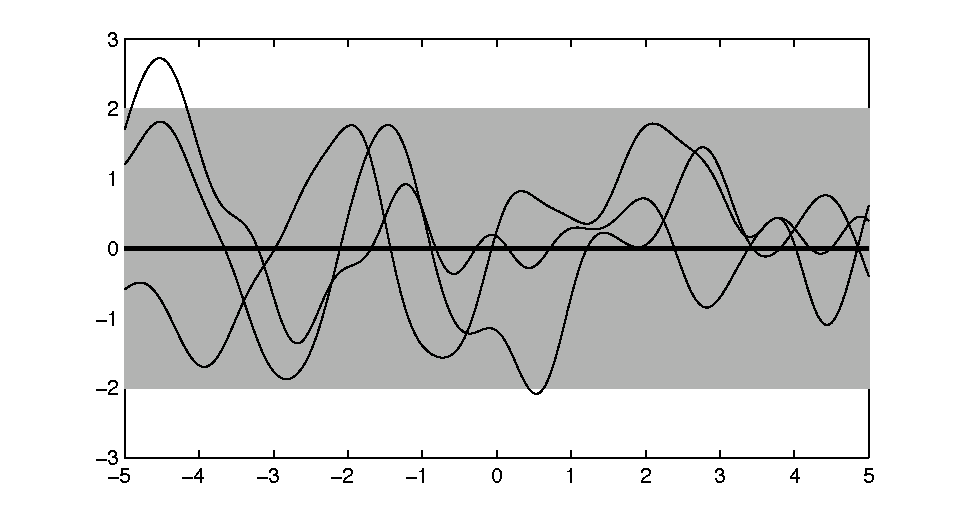
\includegraphics[scale=0.63, clip, trim=2.3cm 1.3cm 2cm 0.9cm]{figs/prior1.pdf}} %rblt
\hfill
\subfigure[Prior samples, $\lambda_2=4\lambda$]{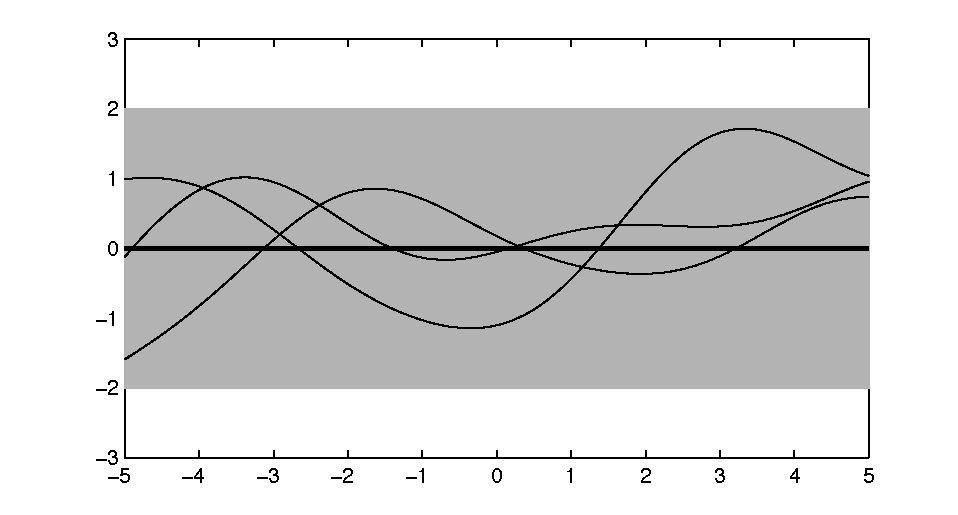
\includegraphics[scale=0.63, clip, trim=2.3cm 1.3cm 2cm 0.9cm]{figs/prior2.pdf}}
\subfigure[Posterior samples, $\lambda_1=\lambda$]{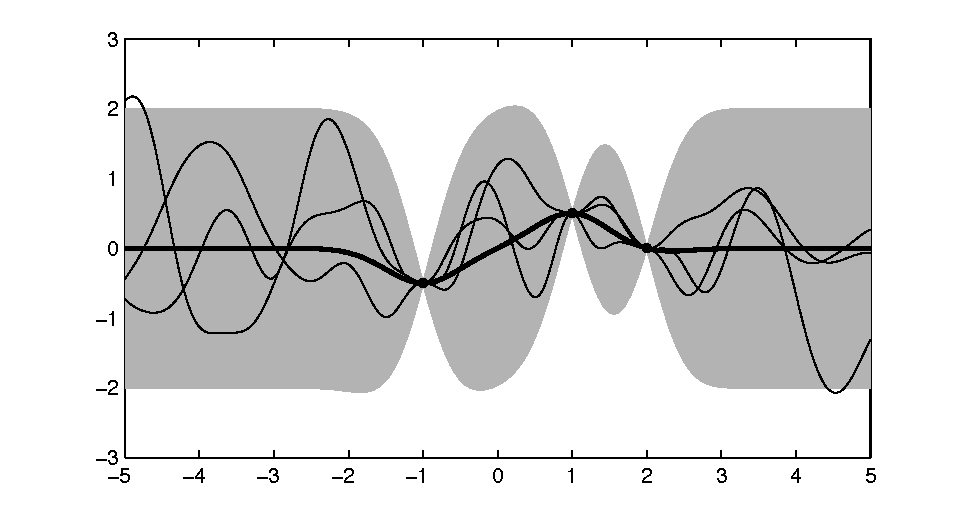
\includegraphics[scale=0.63, clip, trim=2.3cm 1.3cm 2cm 1.5cm]{figs/posterior1.pdf}} %rblt
\hfill
\subfigure[Posterior samples, $\lambda_2=4\lambda$]{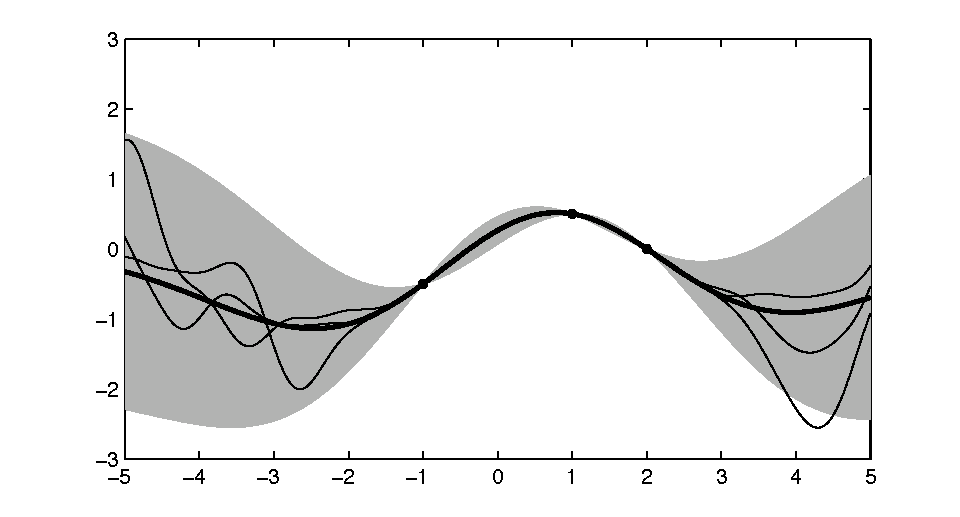
\includegraphics[scale=0.63, clip, trim=2.3cm 1.3cm 2cm 1.5cm]{figs/posterior2.pdf}}
\caption{\small An illustration of the effect of varying the length-scale parameter $\lambda$ in the GP with covariance function $k(x,x') = \exp\left(-\tfrac{1}{2}(x-x')^2/\lambda^2\right)$ and zero mean. Plots (a) and (b) show samples taken from the GP prior before data has been observed. Plots (c) and (d) show samples taken from the posterior after three data points have been observed. The thick black lines show the mean prediction and the grey area depicts the $2\sigma$ or 95\% confidence region.}
\label{lengthsca}
\end{figure}


The squared exponential covariance function \eqref{SE} encodes a smoothness assumption about the underlying function and has useful analytical properties when it comes to making predictions from uncertain inputs (see Section 2.3.2). The hyperparameters in the case of this covariance function are $\boldsymbol{\theta}=[\lambda_{1}\dots \lambda_{N},\alpha,\sigma_\epsilon]^\top$. The covariance matrix $K(X,X)$ or $K$ is defined as the matrix where each element takes on the value $K_{ij}=k(\bx_i,\bx_j)$, $i,j \in \{1\dots n\}$ where $\bx_i,\bx_j \in \mathcal{D}$. It should be noted that there are many different choices of covariance function, the only restriction is that they must produce a symmetric and positive definite covariance matrix $K$.



In a fully Bayesian framework the model would be learned by evaluating the posterior \eqref{posterior} distribution over the function space. This can be done by conditioning on the hyperparameters~$\boldsymbol{\theta}$ to obtain $p(h|\mathbf{y},X)=p(h|\mathbf{y},X,\boldsymbol{\theta})p(\boldsymbol{\theta}|\mathbf{y},X)$ assuming a fixed model structure (fixed covariance function). The posterior $p(h|\mathbf{y},X,\boldsymbol{\theta})$ can be found through Bayes' rule as
\begin{equation}
p(h|\mathbf{y},X,\boldsymbol{\theta}) = 
\frac{p(\mathbf{y}|h,X,\boldsymbol{\theta})p(h|\boldsymbol{\theta})}
        {p(\mathbf{y}|X,\boldsymbol{\theta})},
\end{equation}
where the normalisation constant is obtained through $p(\mathbf{y}|X,\boldsymbol{\theta})=\int p(\mathbf{y}|h,X,\boldsymbol{\theta})p(h|\boldsymbol{\theta})\mathrm{d}h$ with $h \sim \mathcal{GP}$. This can be evaluated analytically since the prior is Gaussian $h|\boldsymbol{\theta} \sim \mathcal{N}(\mathbf{0},K)$ and the likelihood is a factorized Gaussian $\mathbf{y}|h,\boldsymbol{\theta},X \sim \mathcal{N}(h|\boldsymbol{\theta},\sigma^2_\epsilon I)$ because of the assumption of independent noise terms. Now the posterior on the hyperparameters $p(\boldsymbol{\theta}|\mathbf{y},X)$ can similarly be evaluated through Bayes' rule
\begin{equation}
p(\boldsymbol{\theta}|\mathbf{y},X) = 
\frac{p(\mathbf{y}|X,\boldsymbol{\theta})p(\boldsymbol{\theta})}
        {p(\mathbf{y}|X)},
\end{equation}
where the normalisation constant is obtained by integrating out $\boldsymbol{\theta}$, $p(\mathbf{y}|X)=\int p(\mathbf{y}|X,\boldsymbol{\theta})p(\boldsymbol{\theta})\mathrm{d}\boldsymbol{\theta}$. Unfortunately this integral is analytically intractable in most cases of interest. However, a point estimate $\boldsymbol{\hat{\theta}}$ can be found by resorting to optimisation and maximizing the marginal likelihood $p(\mathbf{y}|X,\boldsymbol{\theta})$ with respect to the hyperparameters. For optimisation it is easier to work with the log-marginal likelihood. The analytical expression for this can be found as
\begin{equation}\label{logmarlik}
\mathcal{L}(\boldsymbol{\theta})=\log p(\mathbf{y}|X,\boldsymbol{\theta}) = 
-\tfrac{1}{2}\mathbf{y}^\top(K+\sigma^2_\epsilon I)^{-1}\mathbf{y}   
-  \tfrac{1}{2}\log|K+\sigma^2_\epsilon I|   
- \tfrac{n}{2}\log2\pi.
\end{equation}

The terms in Equation \eqref{logmarlik} have readily interpretable meanings. The first term corresponds to a data-fitting term, it penalizes deviations from the training data. The second term essentially penalizes model complexity by keeping values in the covariance matrix small therefore automatically implementing Occam's razor and avoiding overfitting of the data. The third term is a normalization constant. This is in general a non-convex problem therefore a local maximum found using standard gradient-ascent methods usually suffices. Different peaks correspond to slightly different interpretations of the same data.

Now in order to solve the optimisation problem using gradient-ascent methods the partial derivatives of $\mathcal{L}(\boldsymbol{\theta})$ with respect to the hyperparameters $\boldsymbol{\theta}$ are required. These are given by
\begin{equation}
\frac{\partial\mathcal{L}(\boldsymbol{\theta})}{\partial \theta_i} = 
\tfrac{1}{2}\mathbf{y}^\top K_\epsilon^{-1} \frac{\partial K_\epsilon}{\partial \theta_i} K_\epsilon^{-1}\mathbf{y}
- \tfrac{1}{2}\mathrm{tr}\left( K_\epsilon^{-1} \frac{\partial K_\epsilon}{\partial \theta_i} \right),
\end{equation}
where $K_\epsilon = K+\sigma^2_\epsilon I$. This optimisation problem will be solved using the conjugate gradient with line searches method proposed by \cite{Ras96}. For details of the implementation, the reader is directed to Appendix B of this work.



\section{Prediction with Gaussian Processes}
Now that a Gaussian process model has been learned that explains the training data, it would be desirable to make predictions about what the output will be, given a test input $\bx^*$. First the deterministic case shall be considered, then the stochastic case where $\bx^* \sim \mathcal{N}\left(\bmu^*,\mathbf{\Sigma}^*\right)$.

\subsection{Deterministic Input $\bx^*$}
The joint distribution of the observed target values and the function values at a single deterministic test location $\bx^*$ under the prior can be expressed as
\begin{equation}
\begin{bmatrix}
\mathbf{y} \\
h^*
\end{bmatrix}
\sim \mathcal{N}\left(\mathbf{0},
\begin{bmatrix}
K+\sigma^2_\epsilon I & \bk(\bx^*) \\
\bk(\bx^*)^\top & k(\bx^*)
\end{bmatrix}
\right)
\end{equation}
where $\bk(\bx^*)=K(X,\bx^*) \in \mathbb{R}^n$ and $k(\bx^*)=k(\bx^*,\bx^*) \in \mathbb{R}$. The conditional distribution $h^*|X,\mathbf{y},\bx^* \sim \mathcal{N}\left(\mu(\bx^*),\sigma^2(\bx^*)  \right)$ can then be found using the standard identity for a Gaussian conditional distribution\footnote{
Given $\begin{bmatrix}\bx_a \\ \bx_b\end{bmatrix} \sim \mathcal{N}\left(\begin{bmatrix}\bmu_a \\ \bmu_b\end{bmatrix},\begin{bmatrix}\bSig_a & \bSig_c \\ \bSig_c^\top & \bSig_b\end{bmatrix}  \right)$ then $p(\bx_a|\bx_b) = \mathcal{N}\left( \bmu_b + \bSig_c\bSig_a^{-1}(\bx_a - \bmu_a), \bSig_b - \bSig_c\bSig_a^{-1}\bSig_c^\top  \right)$
} which gives the following solution for prediction at a $\bx^*$
\begin{align}
\mu(\bx^*)&=\boldsymbol{\beta}^\top\bk(\bx^*) \label{mu} \\
\sigma^2(\bx^*)&=k(\bx^*) - \bk(\bx^*)^\top (K+\sigma^2_\epsilon I)^{-1} \bk(\bx^*)  \label{sigma}
\end{align}
where $\boldsymbol{\beta}=(K+\sigma^2_\epsilon I)^{-1}\mathbf{y}$. The general theory of Gaussian process regression as given by these equations was first introduced by \cite{OHa78}. Now a few points should be noted regarding equations \eqref{mu} and \eqref{sigma}. First, the predicted mean $\mu(\bx^*)$ can be interpreted as a weighted sum of the training data targets $\mathbf{y}$. Also, the predicted variance $\sigma^2(\bx^*)$ is unable to exceed the prior variance, $k(\bx^*)=\alpha^2$ in the case of the SE covariance function, since $(K+\sigma^2_\epsilon I)^{-1}$ is positive definite. Finally, it can be seen that inversion of the matrix $(K+\sigma^2_\epsilon I) \in \mathbb{R}^{n \times n}$ is required which has computational complexity of the order $n^3/6$ if the Cholesky factorization method is used. For large data sets this inversion becomes a computationally intensive task and is one of the major drawbacks of Gaussian process regression.

In the case of a multivariate output $\mathbf{y} \in \mathbb{R}^E$, $E$ independent Gaussian process models are trained. The mean and covariance are then given by
\begin{align}
\bmu(\bx^*)&= [ \mu_1(\bx^*)\dots\mu_E(\bx^*) ]^\top , \label{Mu}\\
\bSig(\bx^*)&=\mathrm{diag} \left( \sigma_1^2(\bx^*)\dots\sigma_E^2(\bx^*) \right), \label{Sigma}
\end{align}
respectively. This may seem like an inefficient method of prediction as any potential correlation between outputs is ignored, however within the Gaussian process framework, no better solution has yet been presented.





\subsection{Stochastic Input $\bx^* \sim \mathcal{N}$}

Prediction of the output distribution given an input distribution of $\bx^* \sim \mathcal{N}\left(\bmu^*,\mathbf{\Sigma}^*\right)$ can be found by evaluating the integral
\begin{equation} \label{stocint}
p(h(\bx^*)|\bmu^*,\mathbf{\Sigma}^*,\mathcal{D}) = \int p(h(\bx^*)|\bx^*,\mathcal{D})p(\bx^*)\mathrm{d} \bx^*,
\end{equation}
where $h(\bx^*)|\bx^*,\mathcal{D} \sim \mathcal{N}\left(\mu(\mathbf{x^*}),\sigma^2(\mathbf{x^*})\right)$. Since this is analytically intractable there are two approaches that could be adopted. One possibility is to perform a numerical approximation of this integral by simple Monte Carlo. Alternatively the output distribution can be approximated as a Gaussian and an analytical solution can be obtained. Within this approach there are two possible routes. The first would be to approximate $\mu(\bx^*)$ and $\sigma^2(\bx^*)$ by their Taylor expansions around $\bmu^*$. The second, which is only possible if the squared exponential or a linear covariance function is used, is to evaluate the mean and variance of the output distribution exactly and approximate this with a Gaussian, thereby minimizing the Kullback-Leibler divergence (see \cite{KL51}) between the real and approximate distributions. The approximation of the output of a GP given a stochastic input is illustrated in Figure~\ref{COOLfig}.

The details of the Gaussian approximation methods are outlined in the following sections. Both of these methods rely on the law of iterated expectations and law of conditional variances which are given as
\begin{align}
m(\bx^*) &= \EE_{\bx^*}[\EE_{h(\bx^*)}  [h(\bx^*)|\bx^*]  ] \\
\nonumber&= \EE_{\bx^*}[\mu(\bx^*)], \\
v(\bx^*)  &= \EE_{\bx^*}[\mathrm{var}_{h(\bx_*)}[h(\bx^*)|\bx^*]] + \mathrm{var}_{\bx^*} [\EE_{h(\bx^*)}  [h(\bx^*)|\bx^*]]  \\
\nonumber&=  \EE_{\bx^*}[\sigma^2(\bx^*)]  +  \mathrm{var}_{\bx^*}[\mu(\bx^*)] \\
\nonumber&=  \EE_{\bx^*}[\sigma^2(\bx^*)]  +  \EE_{\bx^*}[\mu(\bx^*)^2]  - \EE^2_{\bx^*}[\mu(\bx^*)],
\end{align}
respectively, where $\EE_{\bx^*}$ and $\mathrm{var}_{\bx^*}$ indicate the expectation and variance under $\bx^*$. For the multivariable case, these results extend to give the following equations
\begin{align}
\mathbf{m}(\bx^*) &= \EE_{\bx^*}[\bmu(\bx^*)], \\
\mathbf{v}(\bx^*)  &=  \EE_{\bx^*}[\bSig(\bx^*)]  +
\EE_{\bx^*}[\bmu(\bx^*)\bmu(\bx^*)^\top]  - 
\EE_{\bx^*}[\bmu(\bx^*)]\EE_{\bx^*}[\bmu(\bx^*)]^\top.
\end{align}
It should be noted that $\Sigma_{ij}=0$ for $i \neq j$ because an independent GP model for each output has been learned.



\begin{figure}[t]
\centering
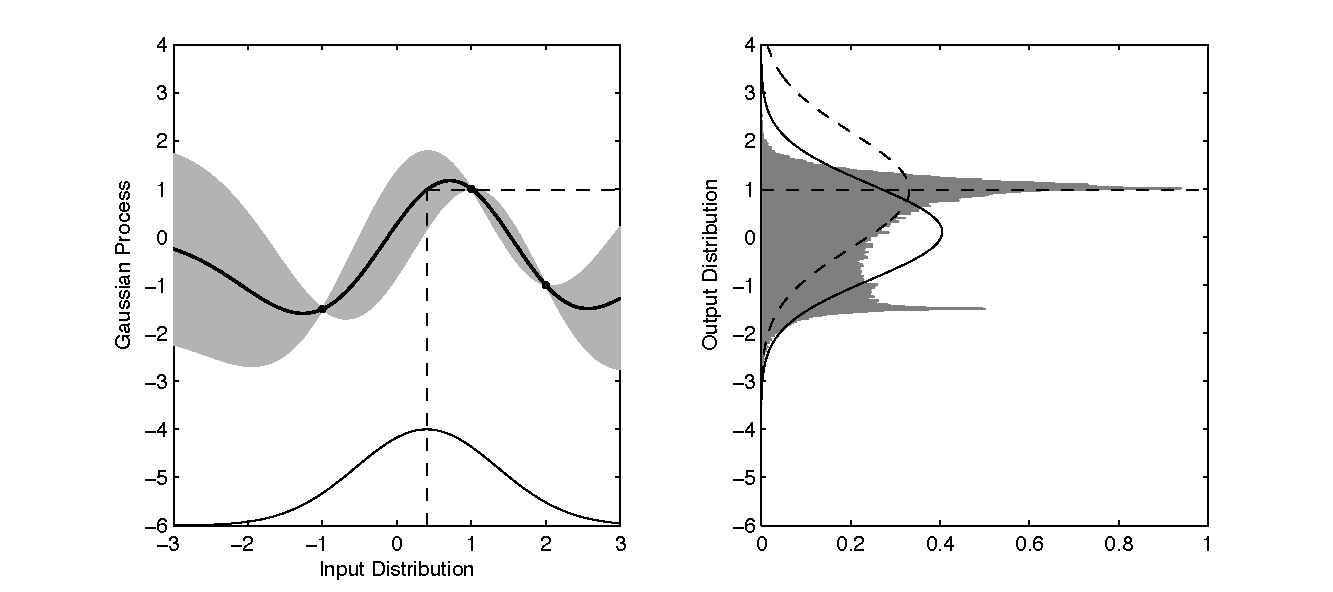
\includegraphics[scale=.75, clip, trim = .5cm 0cm 0cm 0cm]{figs/propunc.pdf}
\caption{\small Illustration of the output distribution of a GP given stochastic input $\bx^* \sim \mathcal{N}\left(\bmu^*,\mathbf{\Sigma}^* \right)$. The left hand plot depicts the unnormalised input distribution at the bottom and the GP at the top, with the grey area representing the $2\sigma$ region. The right hand plot shows the histogram of Monte Carlo samples taken from the input distribution and subsequently sampled from the GP output distribution. A Gaussian approximation calculated by exact moment matching is shown by the solid blue and the Taylor series approximation is shown by the dashed line. The mean prediction of the input mean $\mu(\bmu^*)$ is depicted by a dashed line.}
\label{COOLfig}
\end{figure}



\subsubsection{Taylor Series Approximation}
Following the detailed calculations given in the thesis by \cite{GRM02} it is shown that, within a first order Taylor expansion of the mean prediction and a second order expansion of the variance\footnote{Mixed expansions were used in order to keep the $\mathrm{var}_{\bx^*}[\mu(\bx^*)]$ term in the variance manageable.} the following expressions are obtained
\begin{align} 
m(\bx^*) &\approx
\overbrace{
\mu(\bmu^*)
}^{\EE_{\bx^*}[\mu(\bx^*)]},  \label{taylormean}\\
v(\bx^*) &\approx
\underbrace{
\sigma^2(\bmu^*)  +
\frac{1}{2}\mathrm{tr} \left( \mathbf{\Sigma}^*
\left.\frac{\partial^2\sigma^2(\bx^*)}{\partial\bx^*\partial\bx^{*\top}}\right|_{\bx^*=\bmu^*} \right)
}_{\EE_{\bx^*}[\sigma^2(\bx^*)]}  +
\underbrace{
\left.\frac{\partial\mu(\bx^*)}{\partial\bx^*}\right|_{\bx^*=\bmu^*}^\top
\!\!\!\!\!\!\!\mathbf{\Sigma}^*
\left.\frac{\partial\mu(\bx^*)}{\partial\bx^*}\right|_{\bx^*=\bmu^*}
}_{\mathrm{var}_{\bx^*}[\mu(\bx^*)]} ,  \label{taylorvar}
\end{align}
where $\mu$ and $\sigma^2$ are given by the expressions for a deterministic input, Equations~\eqref{mu} and \eqref{sigma} respectively. As can be seen in Figure~\ref{COOLfig} this method provides no corrective term for the mean prediction. In the case of the squared exponential covariance function plus a noise term, the elements of the partial derivatives are given by
\begin{align}
\left.\frac{\partial\mu(\bx^*)}{\partial x^*_{i}}\right
|_{\bx^*=\bmu^*} 
&=
\frac{\partial \bk(\bmu^*)}{\partial x^*_{i}}^\top
K_\epsilon^{-1} \mathbf{y}, 
\\
\left.\frac{\partial^2\sigma^2(\bx^*)}{\partial x^*_{i}\partial x^*_{j}}\right
|_{\bx^*=\bmu^*} 
&=
\frac{\partial^2 k(\bmu^*)}{\partial x^*_{i}\partial x^*_{j}} - 
2\frac{\partial \bk(\bmu^*)}{\partial x^*_{i}}^\top
K_\epsilon^{-1}
\frac{\partial \bk(\bmu^*)}{\partial x^*_{j}} - 
2\frac{\partial^2 \bk(\bmu^*)}{\partial x^*_{i}\partial x^*_{j}}^\top
K_\epsilon^{-1}
\bk(\bmu^*),
\end{align}
where in the case of the squared exponential covariance function, the $k(\cdot)$ and $\bk(\cdot)$ derivatives are given by
\begin{align}
\frac{\partial^2 k(\bmu^*)}{\partial x^*_{i}\partial x^*_{j}}
&= \frac{\partial^2 k(\bmu^*)}{\partial x^*_{i}} = 0,
\\
\frac{\partial \bk(\bmu^*)}{\partial x^*_{i}}
&=
A_i  \circ  \bk(\bmu^*),
\\
\frac{\partial^2 \bk(\bmu^*)}{\partial x^*_{i}\partial x^*_{j}}
&=
\left[-\tfrac{1}{\lambda_i^2}\delta_{ij}\mathbf{1} + A_i \circ A_j  \right] \circ
\bk(\bmu^*),
\end{align}
where $A_i = \tfrac{1}{\lambda_i^2}(X_{(i:)}^\top - {\mu^*_{(i)}}\mathbf{1}) \in \mathbb{R}^{n}$, the indices $i,j \in \{1\dots N\}$, $\delta_{ij}$ is the Kronecker delta, $\mathbf{1}$ is an $n$-dimensional vector of $1$'s, $X_{(i:)}$ is the $i^{\text{th}}$ row of the input data matrix $X$ and $\circ$ denotes the Hadamard product. The elements of the multivariate mean $\mathbf{m}$ and corresponding covariance matrix $\mathbf{v}$ can be found by a simple extension to the univariate case as
\begin{align} 
m_a(\bx^*) &\approx  \mu_a(\bmu^*) \label{TaylorM}\\
v_{ab}(\bx^*) &\approx  \left[
\sigma_a^2(\bmu^*)  + 
\frac{1}{2}\mathrm{tr} \left( \mathbf{\Sigma}^*
\left.\frac{\partial^2\sigma_a^2(\bx^*)}{\partial\bx^*\partial\bx^{*\top}}\right|_{\bx^*=\bmu^*} \right) \right] \delta_{ab}  
+
\left.\frac{\partial\mu_a(\bx^*)}{\partial\bx^*}\right|_{\bx^*=\bmu^*}^\top
\!\!\!\!\!\!\!\mathbf{\Sigma}^*
\left.\frac{\partial\mu_b(\bx^*)}{\partial\bx^*}\right|_{\bx^*=\bmu^*}.   \label{TaylorV}
\end{align}







\subsubsection{Exact Moment Matching Approximation}
The detailed derivation of this approach can be found in \cite{QGR03}, or \cite{QGLR03} for an overview of the results. The key step proposed by the authors is noticing that the squared exponential covariance function \eqref{SE} is essentially an un-normalized Gaussian distribution. Therefore by using the product of Gaussian densities\footnote{
Given by $\mathcal{N}(\bmu_a,\bSig_a).\mathcal{N}(\bmu_b,\bSig_b) = z_c\mathcal{N}(\bmu_c,\bSig_c)$ where $\bmu_c = (\bSig_a^{-1} + \bSig_b^{-1})^{-1}(\bSig_a^{-1}\bmu_a + \bSig_b^{-1}\bmu_b)$, $\bSig_c = (\bSig_a^{-1} + \bSig_b^{-1})^{-1}$ and $z_c = |2\pi(\bSig_a + \bSig_b)|^{-\tfrac{1}{2}} \exp\left(-\tfrac{1}{2}(\bmu_a - \bmu_b)^\top(\bSig_a + \bSig_b)^{-1}(\bmu_a - \bmu_b) \right)$.
} the mean and variance of the integral \eqref{stocint} can be evaluated exactly. Then fitting a Gaussian distribution to these moments gives an estimate of the output distribution. The mean and variance for the univariate case are given by
\begin{align}
m(\bx^*) &=  \overbrace{\boldsymbol{\beta}^\top \mathbf{q}}^{\EE_{\bx^*}[\mu(\bx^*)]}, \label{unimean}\\
v(\bx^*) &= \underbrace{\alpha^2 - \mathrm{tr}\left( (K+\sigma^2_\epsilon I)^{-1} \mathbf{Q}  \right)}_{\EE_{\bx^*}[\sigma^2(\bx^*)] }
+ \underbrace{\boldsymbol{\beta}^\top \mathbf{Q} \boldsymbol{\beta} }_{\EE_{\bx^*}[\mu(\bx^*)^2]} 
- \underbrace{ \boldsymbol{\beta}^\top (\mathbf{q} \mathbf{q}^\top) \boldsymbol{\beta}}_{\EE^2_{\bx^*}[\mu(\bx^*)]}, \label{univar}
\end{align}
respectively, where the elements of $\mathbf{q}$ and $\mathbf{Q}$ are given by
\begin{align}
q_i &= \alpha^2 \left|\bLam^{-1}\mathbf{\Sigma}^* + I  \right|^{-\tfrac{1}{2}} 
\exp \left(-\tfrac{1}{2} (\bmu^*  -  \bx_i)^\top  (\bLam + \mathbf{\Sigma}^*)^{-1}  (\bmu^*  -  \bx_i)     \right),  \\
 Q_{ij} 
&= k_i k_j \left|2\bLam^{-1}\mathbf{\Sigma}^* + I  \right|^{-\tfrac{1}{2}} \exp  \left( 2(\bmu^*  -  \mathbf{\hat x}_{ij})^\top \bLam^{-1} (2\bLam^{-1} + \mathbf{\Sigma}^{*-1})^{-1}  \bLam^{-1}  (\bmu^*  -  \mathbf{\hat x}_{ij}) \right),
\end{align}
where $\mathbf{\hat x}_{ij} = \tfrac{1}{2}(\bx_i + \bx_j)$ and $k_i$ is the $i^{th}$ element of $\bk(\bmu^*)$. This method is similarly depicted in Figure~\ref{COOLfig} with a much closer approximation to the true distribution. It should be noted that as $\mathbf{\Sigma}^*  \rightarrow \mathbf{0}$, $\mathbf{q} \rightarrow \bk$ and $\mathbf{Q} \rightarrow  \mathbf{kk}^\top$ so Equations \eqref{unimean} and \eqref{univar} reduce to the deterministic equations \eqref{mu} and \eqref{sigma}. Also, a key difference between the mean predicted by moment matching \eqref{unimean} and the mean predicted through Taylor expansion \eqref{taylormean} is that $\bk$ has been augmented by the input variance $\mathbf{\Sigma}_{\bx^*}$ to give $\mathbf{q}$.

The extension to the multivariable case can be found in the thesis by \cite{Dei09}. The elements of the mean $\mathbf{m}$ and covariance matrix $\mathbf{v}$ can be written succinctly as
\begin{align}
m_a(\bx^*) &= \boldsymbol{\beta}_a^\top \mathbf{q}_a, \label{MMM}\\
v_{ab}(\bx^*) &=
\left[ \alpha_a^2 - \mathrm{tr}\left( (K+\sigma^2_{\epsilon a} I)^{-1} \mathbf{Q}  \right) \right] \delta_{ab} +
\boldsymbol{\beta}^\top_a\mathbf{Q} \boldsymbol{\beta}_b -
\boldsymbol{\beta}^\top_a (\mathbf{q}_a \mathbf{q}_b^\top) \boldsymbol{\beta}_b, \label{MMV}
\end{align}
where now the elements of $\mathbf{Q}$ are given by
\begin{align}
\label{Qdef}
Q_{ij} =&\: k^a_i k^b_j
\left|(\bLam_a^{-1} + \bLam_b^{-1})
        \mathbf{\Sigma}^* + I  \right|^{-\tfrac{1}{2}} \\
\nonumber&\quad \exp  \left( 
2(\bmu^*  -  \mathbf{\hat x}_{ij})^\top \bLam_a^{-1}
\left((\bLam_a^{-1} + \bLam_b^{-1}) + 
\mathbf{\Sigma}^{*-1}\right)^{-1}  \bLam_b^{-1}
(\bmu^*  -  \mathbf{\hat x}_{ij}) \right),
\end{align}
where $\mathbf{\hat x}_{ij} = \bLam_b(\bLam_a + \bLam_b)^{-1}\bx_i + \bLam_a(\bLam_a + \bLam_b)^{-1}\bx_j$. This concludes the outline of how to make predictions about the values of unknown functions given deterministic or stochastic inputs using GP models. How this capability can be used to model the behaviour of dynamic systems is the subject of the following section.




\section{Modelling Dynamics and Multiple-step Ahead Prediction}
Returning attention to the discrete time dynamic system described by Equation~\eqref{system}, $N$ independent Gaussian process models can be trained to learn these dynamics given training data of the form $\mathcal{D}=\{[\bx_{t_i}^\top \:\mathbf{u}_{t_i}^\top]^\top, \bx_{t_i+1} | i=1\dots n \}$. In essence, the mapping from the current state $\bx_k$ and input $\mathbf{u}_k$ to the next state $\bx_{k+1}$ is learned. Now given some current state $\bx_k$, deterministic or stochastic, a prediction about the what the next state $\bx_{k+1}$ will be can be made, given either a deterministic input or a distribution over input space. This setup allows multiple step ahead predictions to be made in an iterative fashion. The advantage of this framework is that the state uncertainty is propagated in the prediction along with the mean, instead of just na\"{i}vely discarding the variance and using only the mean for prediction. Another approach is to directly learn the gradient of the dynamics, where instead of predicting the value of $\bx_{k+1}$, the value of $\Delta\bx_k = \bx_{k+1} - \bx_k$ is predicted.


\section{Learning Policies}
{\hl Mention that we ideally want to condition on previous states to give consistency in dynamics...but impossible, so assume timestep is long enough!}


\section{Summary}
This chapter has introduced the Gaussian process modelling framework for dynamic systems. Gaussian processes are a nonparametric modelling technique that formally incorporates uncertainty information into its predictions. When making predictions given a distribution over inputs, the output distribution can be approximated as a Gaussian using either the technique of Taylor series expansions or exact moment matching. Gaussian processes can also be used in the context of filtering in partially observable systems using approximations to the optimal Bayes' filter.

